\documentclass[a4paper]{article}
\usepackage[affil-it]{authblk}
\usepackage[english]{babel}
\usepackage[backend=bibtex,style=numeric]{biblatex}

\usepackage{geometry}
\geometry{margin=1.5cm, vmargin={0pt,1cm}}
\setlength{\topmargin}{-1cm}
\setlength{\paperheight}{29.7cm}
\setlength{\textheight}{25.3cm}

% useful packages.
\usepackage{amsfonts}
\usepackage{amsmath}
\usepackage{amssymb}
\usepackage{amsthm}     
\usepackage{abstract}
\usepackage{booktabs}
\usepackage{enumerate} %enumerate environment
\usepackage{graphicx}
\usepackage{multicol}
\usepackage{fancyhdr}
\usepackage{url}
\usepackage{multirow}
\usepackage{amsfonts}
\usepackage{mathrsfs}
\usepackage{upgreek}
\usepackage{caption}
\usepackage{subcaption}
\usepackage{layout}
\usepackage{ctex}      %中文环境
\usepackage{booktabs}  %三线表
\usepackage{verbatim}  %comment environment
\usepackage{float}     %强制表格图片位置
\usepackage{listings}  %insert code in latex
\usepackage{fontspec}  %font support
\usepackage{tikz}
\usetikzlibrary{shapes, arrows}
\usepackage{makecell}
\usetikzlibrary{intersections}
\usepackage{arydshln}


\usepackage[colorlinks,linkcolor=blue]{hyperref}
\usepackage{xcolor}
\definecolor{mygreen}{rgb}{0,0.6,0}
\definecolor{lightgrey}{rgb}{0.95,0.95,0.95}
\definecolor{winered}{rgb}{0.5,0,0}
\definecolor{mymauve}{rgb}{0.58,0,0.82}
\lstset{
      backgroundcolor=\color{lightgrey},
      basicstyle             = \ttfamily,
      breakatwhitespace      = false,
      breaklines             = true,
      captionpos             = none,
      commentstyle           = \color{mygreen}\bfseries,
      extendedchars          = false,
      keepspaces             = true,
      keywordstyle           = \color{winered},         % keyword style
      language               = python,                     % the language of code
      otherkeywords          = {string},
      numberstyle            = \tiny\color{mygray},
      rulecolor              = \color{black},
      showspaces             = false,
      showstringspaces       = false,
      showtabs               = false,
      stepnumber             = 1,
      stringstyle            = \color{mymauve},         % string literal style
      tabsize                = 2,
      title                  = \lstname,
      aboveskip              = 0pt,
      belowskip              = 0pt,
      columns                = flexible
}

% some common command
\newcommand{\dif}{\mathrm{d}}
\newcommand{\avg}[1]{\left\langle #1 \right\rangle}
\newcommand{\norm}[1]{\left\| #1 \right\|}
\newcommand{\difFrac}[2]{\frac{\dif #1}{\dif #2}}
\newcommand{\pdfFrac}[2]{\frac{\partial #1}{\partial #2}}
\newcommand{\OFL}{\mathrm{OFL}}
\newcommand{\UFL}{\mathrm{UFL}}
\newcommand{\fl}{\mathrm{fl}}
\newcommand{\op}{\odot}
\newcommand{\Eabs}{E_{\mathrm{abs}}}
\newcommand{\Erel}{E_{\mathrm{rel}}}


\begin{document}
% =================================================
\title{Dionysus2 持久同调分析代码文档}

\author{Zhouyue Qian 3220104074
  \thanks{Electronic address: \texttt{3220104074@edu.zju.cn}}}
\affil{(Information and Computational Science Class 2201), Zhejiang University }


\date{Due time: \today}

\maketitle

\section{概述和环境要求}
本代码使用 Dionysus2 库对点云数据进行拓扑数据分析，计算并可视化其持续同调特征。主要功能包括：
\begin{itemize}
    \item 从文本文件读取点云数据
    \item 构建 Rips 复形
    \item 计算持续同调（0 维和 1 维）
    \item 生成持久图（Persistence Diagrams）
    \item 标注关键拓扑特征点
    \item 输出详细的拓扑特征信息
\end{itemize}
运行本代码需要以下 Python 库：
\begin{itemize}
    \item \texttt{dionysus2} (版本 2.0.8 或更高)
    \item \texttt{numpy} (版本 1.21.0 或更高)
    \item \texttt{matplotlib} (版本 3.5.0 或更高)
    \item \texttt{scipy} (版本 1.7.0 或更高)
\end{itemize}
安装命令：
\begin{lstlisting}[language=bash]
pip install dionysus2 matplotlib numpy scipy
\end{lstlisting}

\section{代码结构}

\subsection{主要函数}
\begin{enumerate}
    \item \texttt{read\_points(filename)}: 读取点云数据文件
    
    \begin{itemize}
        \item 输入: 文件名 (如 \texttt{cloud.txt})
        \item 输出: NumPy 数组格式的点坐标
        \item 格式要求: 每行一个点，坐标值用空格分隔
    \end{itemize}

    \item \texttt{plot\_persistence\_diagram(dgm, dim, max\_death, annotate)}: 绘制持久图
    
    \begin{itemize}
        \item \texttt{dgm}: 持续同调图
        \item \texttt{dim}: 同调维度 (0 或 1)
        \item \texttt{max\_death}: 最大死亡时间 (用于绘制对角线)
        \item \texttt{annotate}: 是否标注点信息 (仅用于 H1)
    \end{itemize}

    \item \texttt{main()}: 主程序流程
    
    \begin{itemize}
        \item 读取点云数据
        \item 计算最大距离
        \item 构建 Rips 复形
        \item 计算持续同调
        \item 输出拓扑特征信息
        \item 绘制并保存持久图
    \end{itemize}
\end{enumerate}

\subsection{算法流程}
\begin{enumerate}
    \item 读取点云数据
    \item 计算点云直径: $\max_{i,j} \|p_i - p_j\|$
    \item 设置最大距离阈值: $d_{\max} = \text{diameter} \times 1.3$
    \item 构建 Rips 复形 (维度上限为 2)
    \item 创建过滤复合体并排序
    \item 计算持续同调
    \item 初始化持续图
    \item 输出 H1 特征点信息
    \item 绘制 H0 和 H1 持久图
\end{enumerate}

\section{参数说明}

\subsection{关键参数}
\begin{itemize}
    \item \texttt{max\_distance} 系数 (默认为 1.3)
    
    \begin{itemize}
        \item 控制 Rips 复形的最大半径
        \item 增大值可捕捉更大的拓扑特征，但会增加计算复杂度
        \item 减小值可加速计算，但可能遗漏重要特征
    \end{itemize}

    \item \texttt{max\_dim} (默认为 2)
    
    \begin{itemize}
        \item 构建复形的最高维度
        \item 计算 H1 至少需要维度 2
        \item 计算 H2 需要设置为 3
    \end{itemize}
\end{itemize}

\subsection{输出参数}
\begin{itemize}
    \item \texttt{persistence\_diagrams\_annotated.png} 图像参数:
    \begin{itemize}
        \item 尺寸: 14×6 英寸
        \item 分辨率: 300 DPI
        \item 布局: 左右子图 (H0 和 H1)
    \end{itemize}
    \item 控制台输出:
    \begin{itemize}
        \item 点云直径
        \item H1 特征点详细信息表
    \end{itemize}
\end{itemize}

\section{输出说明}
这里通过\textbf{plot\_raw.py}可以画出\textbf{cloud.txt}的原始图像，展示点云数据的分布情况。
\begin{figure}[h]
  \centering
  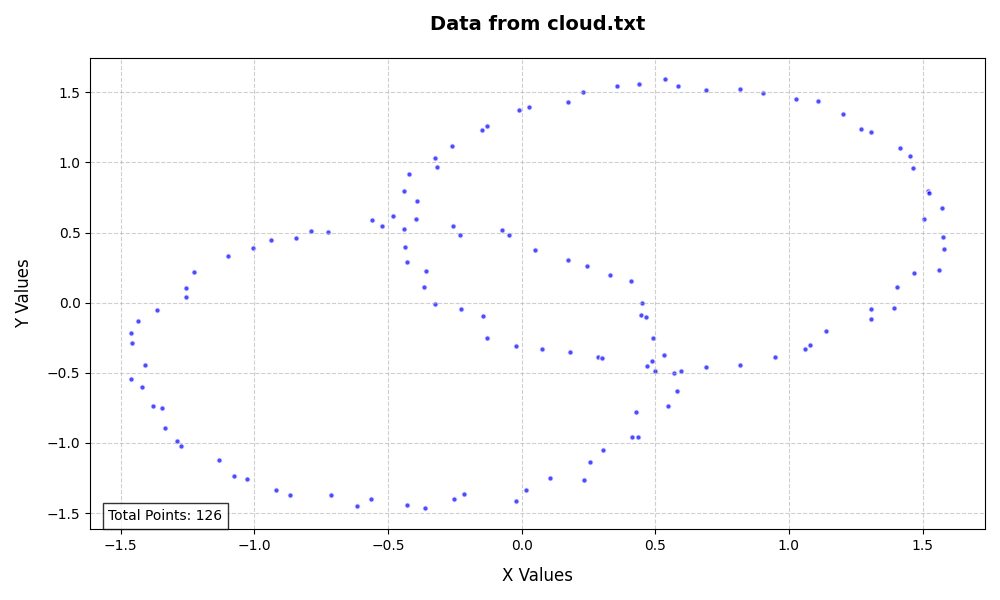
\includegraphics[width=0.8\textwidth]{raw.png}
  \caption{点云数据原始图像}
  \label{fig:cloud_raw}
\end{figure}

\subsection{持久图}
\begin{itemize}
    \item \textbf{H0 图 (左)}: 展示 0 维同调特征
    \begin{itemize}
        \item X 轴: 出生时间 (Birth time)
        \item Y 轴: 死亡时间 (Death time)
        \item 点特征: 沿 X=0 直线分布，代表连通分量
    \end{itemize}
    
    \item \textbf{H1 图 (右)}: 展示 1 维同调特征
    \begin{itemize}
        \item 黑色虚线: 对角线 (y=x)
        \item 点标注:
        \begin{itemize}
            \item 坐标: (出生时间, 死亡时间)
            \item 持续时间: $\Delta = \text{死亡时间} - \text{出生时间}$
            \item 点编号: \#0, \#1, ...
        \end{itemize}
    \end{itemize}
\end{itemize}
\begin{figure}[h]
  \centering
  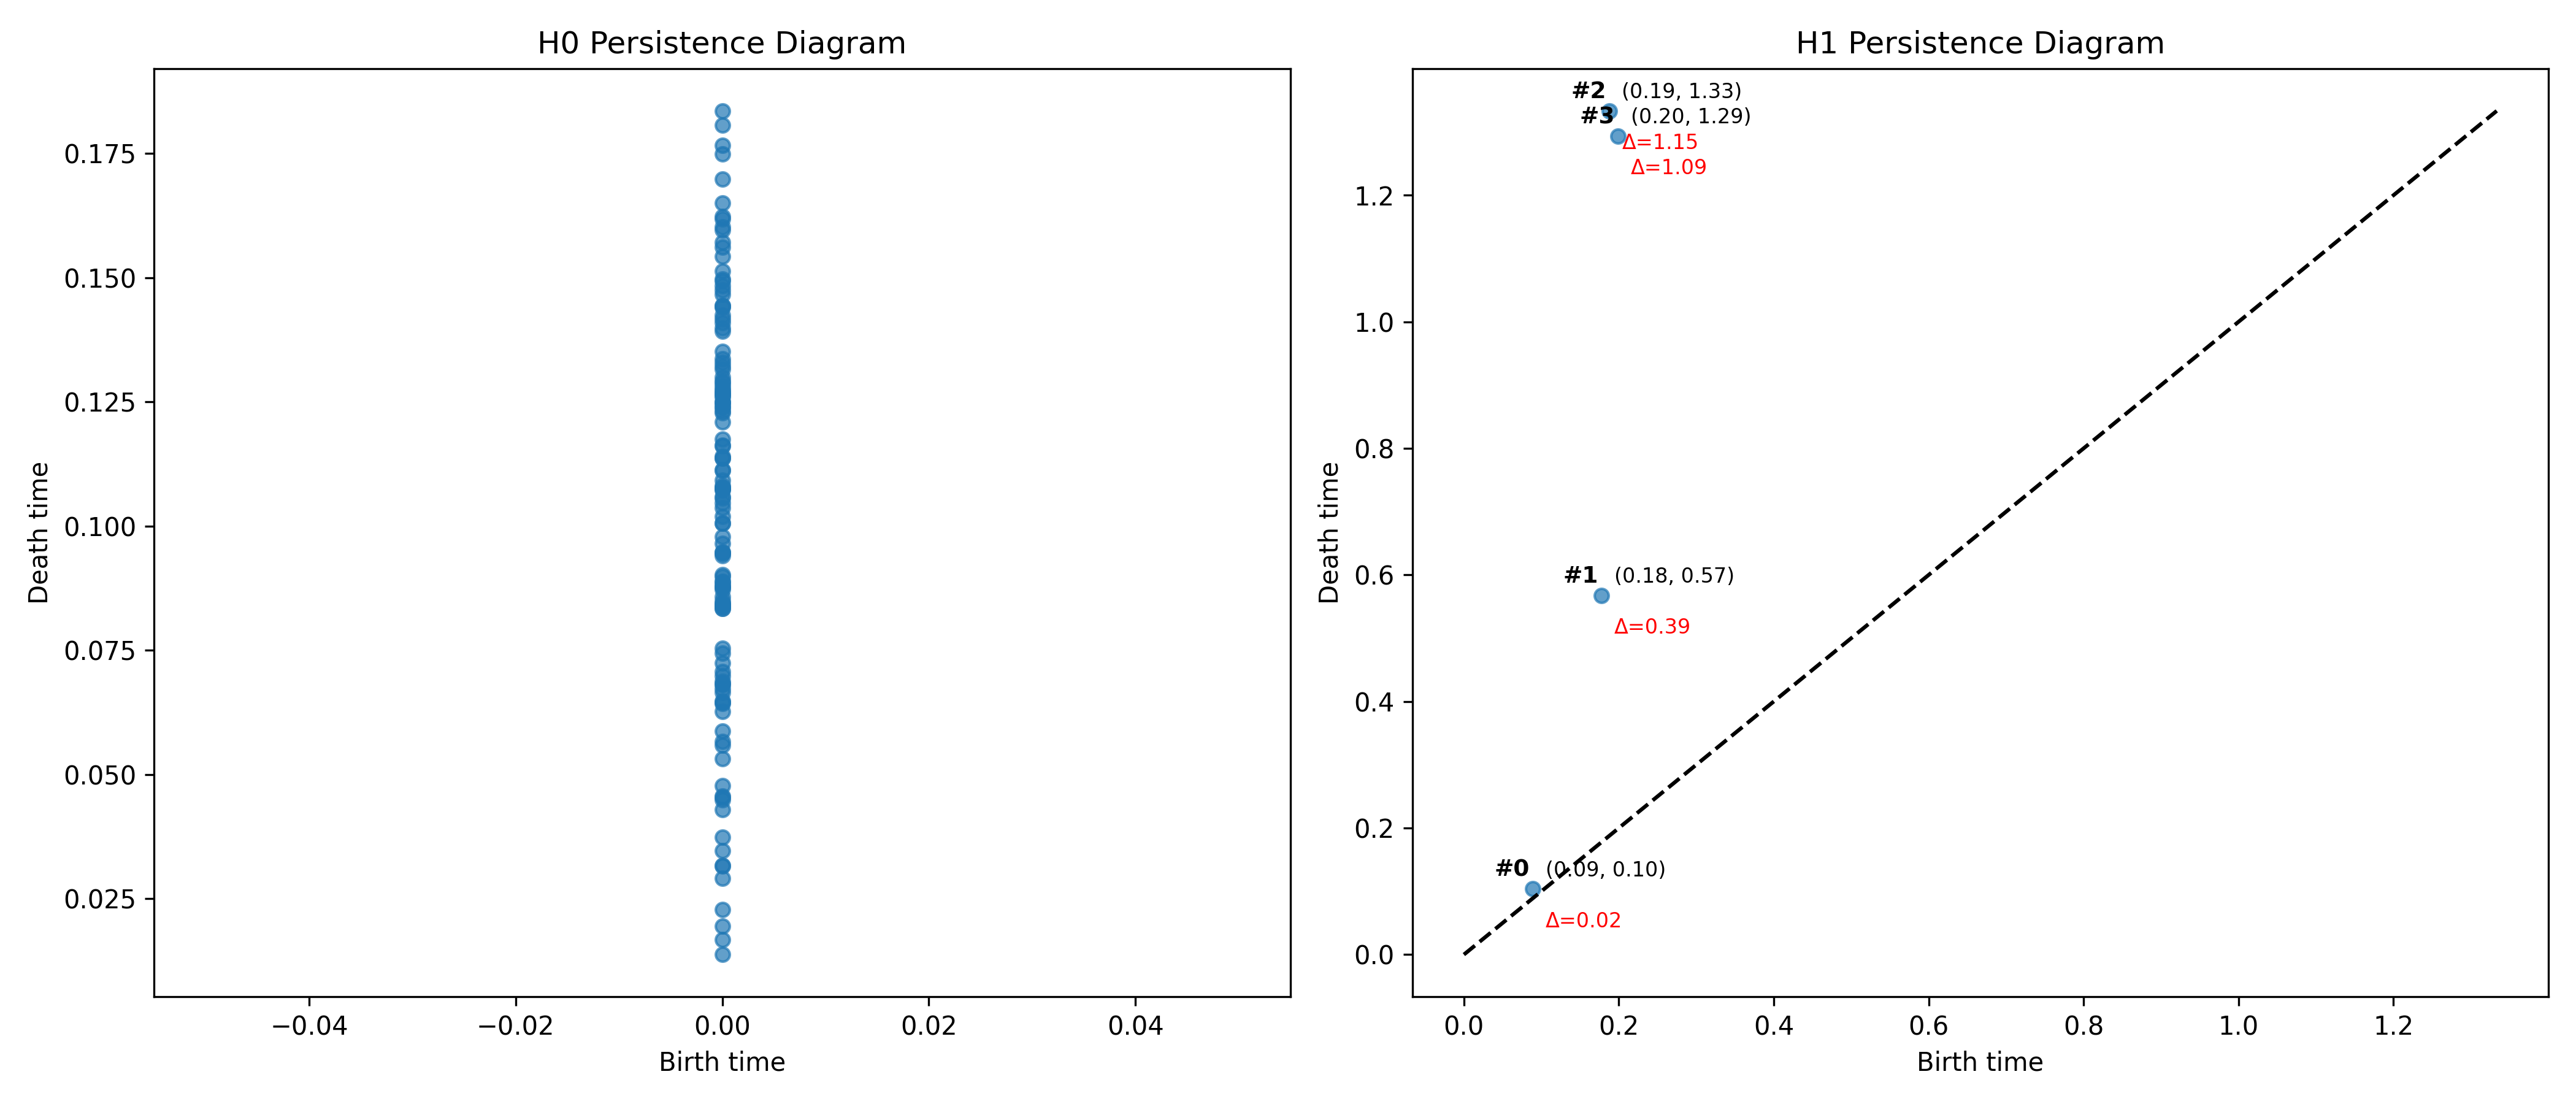
\includegraphics[width=0.8\textwidth]{persistence_diagrams_annotated.png}
  \caption{持久图 (左: H0, 右: H1)}
  \label{fig:persistence_diagram}
\end{figure}

\subsection{控制台输出}
\begin{figure}[h]
  \centering
  
\includegraphics[width=0.8\textwidth]{result.png}
\end{figure}

\end{document}